\begin{figure}[H]
    \centering
    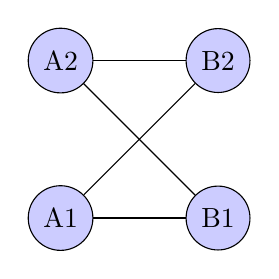
\begin{tikzpicture}
        \node[circle, draw, fill=blue!20] (A1) at (0,0) {A1};
        \node[circle, draw, fill=blue!20] (A2) at (0,2) {A2};
        \node[circle, draw, fill=blue!20] (B1) at (2,0) {B1};
        \node[circle, draw, fill=blue!20] (B2) at (2,2) {B2};
        \draw (A1) -- (B1);
        \draw (A1) -- (B2);
        \draw (A2) -- (B1);
        \draw (A2) -- (B2);
    \end{tikzpicture}
    \caption{Bipartite graph example.}
    \label{fig:bipartite-graph}
\end{figure}